\documentclass{standalone}
\usepackage{tikz}
\usetikzlibrary{patterns, positioning}
\usepackage[sfdefault]{ClearSans} %% option 'sfdefault' activates Clear Sans as the default text font
\usepackage[T1]{fontenc}

\begin{document}
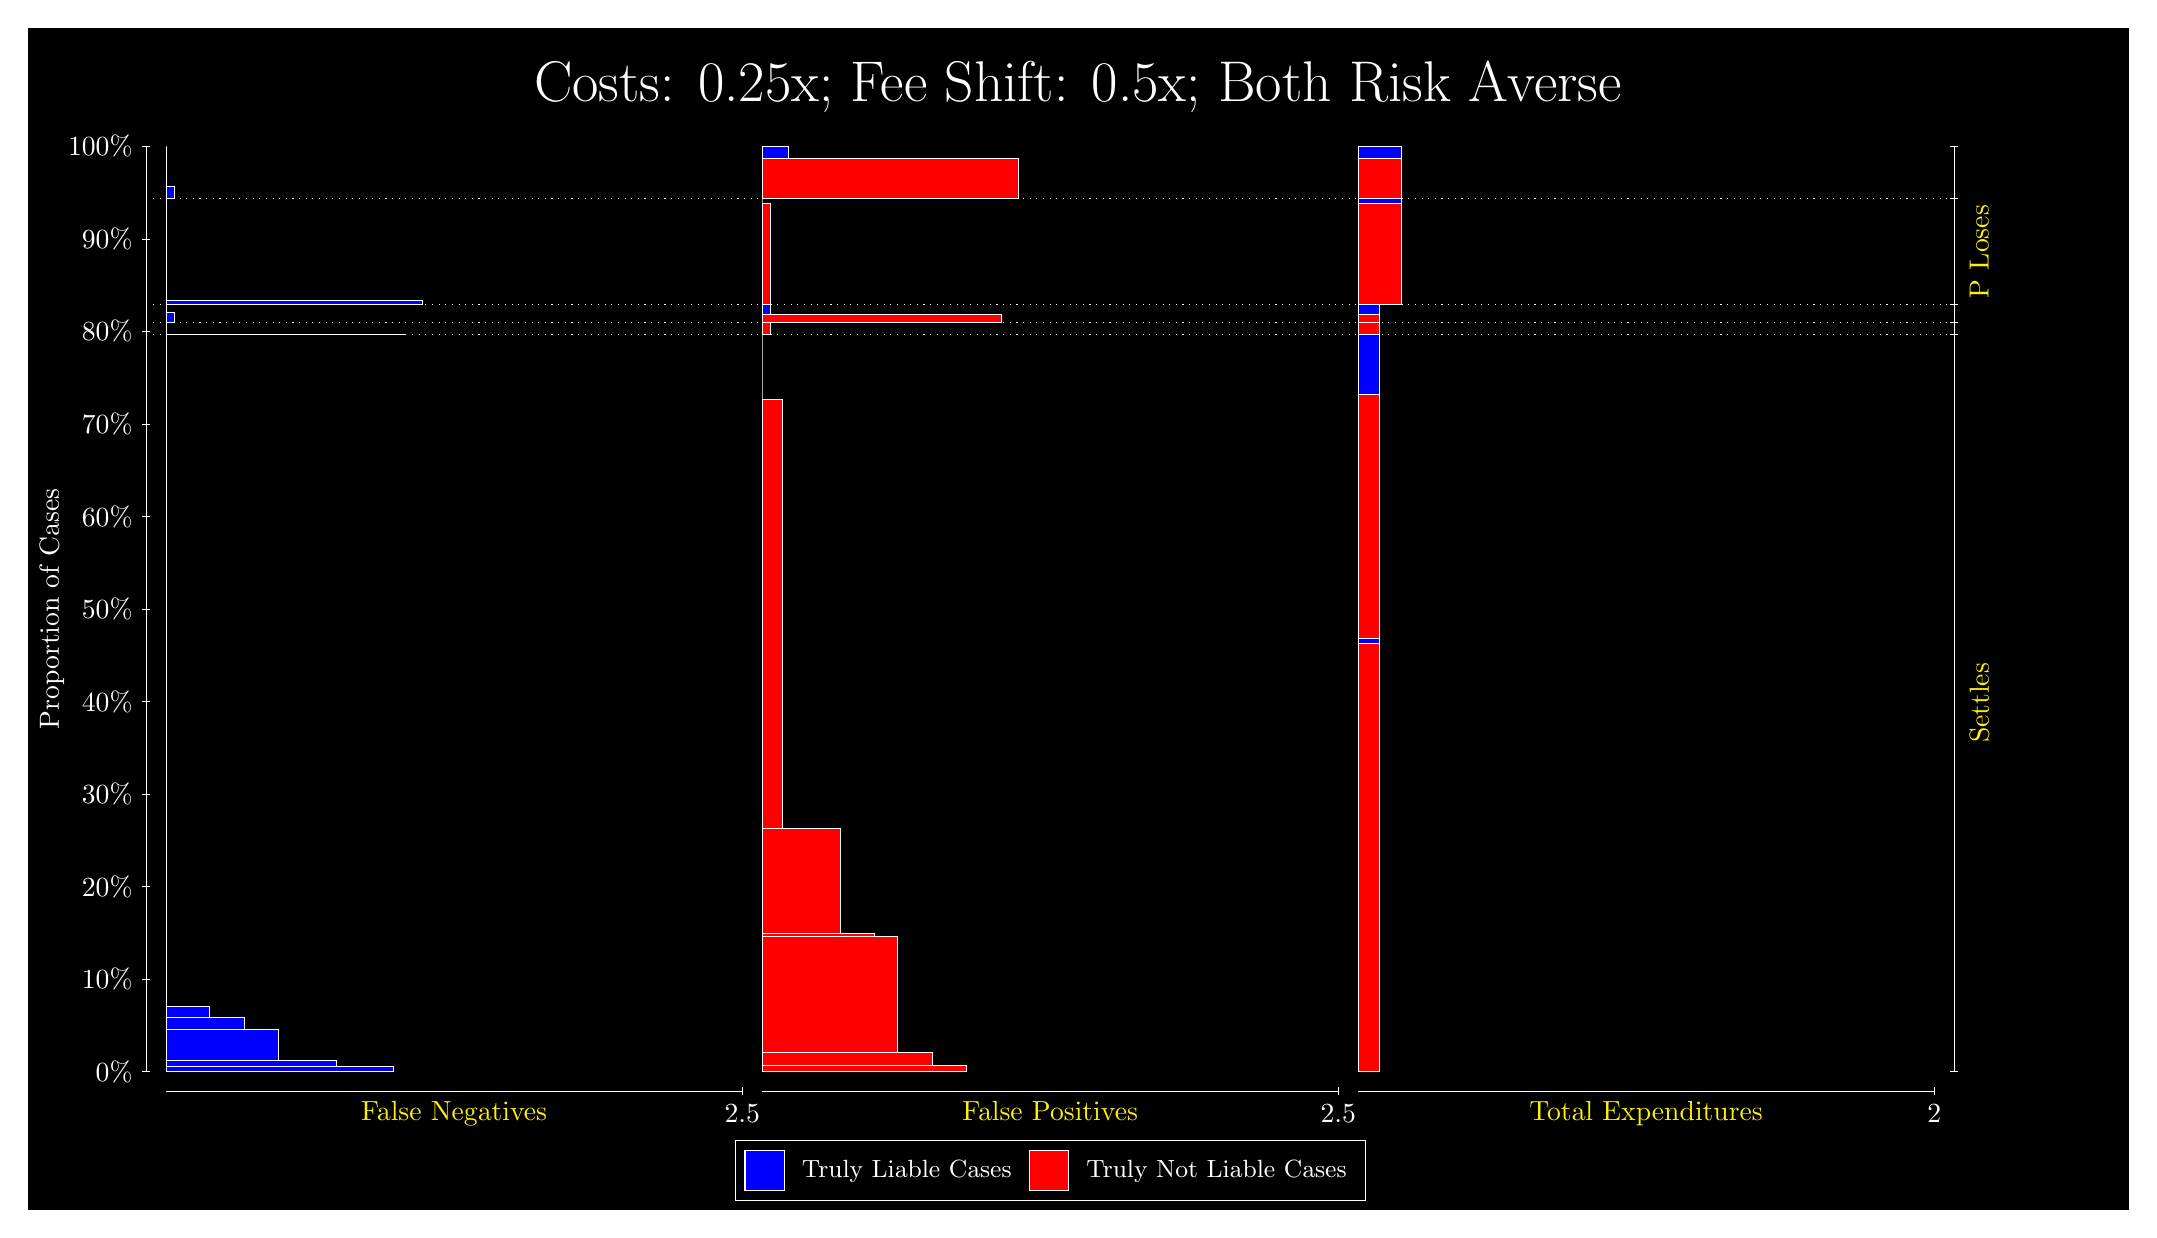
\begin{tikzpicture}
\draw[fill=black] (0,0) rectangle (26.667,15);
\draw[text=white] (0,13.5) rectangle (26.667,15) node[midway] {\huge Costs: 0.25x; Fee Shift: 0.5x; Both Risk Averse};
\draw[white, very thin] (1.5,1.75) -- (1.5,13.5);
\node[rotate=90, text=white, anchor=center] at (0.3, 7.625) {Proportion of Cases};
\draw[white, very thin] (1.45,1.75) -- (1.55,1.75);
\node[text=white, anchor=east] at (1.45, 1.75) {0\%};
\draw[white, very thin] (1.45,2.925) -- (1.55,2.925);
\node[text=white, anchor=east] at (1.45, 2.925) {10\%};
\draw[white, very thin] (1.45,4.1) -- (1.55,4.1);
\node[text=white, anchor=east] at (1.45, 4.1) {20\%};
\draw[white, very thin] (1.45,5.275) -- (1.55,5.275);
\node[text=white, anchor=east] at (1.45, 5.275) {30\%};
\draw[white, very thin] (1.45,6.45) -- (1.55,6.45);
\node[text=white, anchor=east] at (1.45, 6.45) {40\%};
\draw[white, very thin] (1.45,7.625) -- (1.55,7.625);
\node[text=white, anchor=east] at (1.45, 7.625) {50\%};
\draw[white, very thin] (1.45,8.8) -- (1.55,8.8);
\node[text=white, anchor=east] at (1.45, 8.8) {60\%};
\draw[white, very thin] (1.45,9.975) -- (1.55,9.975);
\node[text=white, anchor=east] at (1.45, 9.975) {70\%};
\draw[white, very thin] (1.45,11.15) -- (1.55,11.15);
\node[text=white, anchor=east] at (1.45, 11.15) {80\%};
\draw[white, very thin] (1.45,12.325) -- (1.55,12.325);
\node[text=white, anchor=east] at (1.45, 12.325) {90\%};
\draw[white, very thin] (1.45,13.5) -- (1.55,13.5);
\node[text=white, anchor=east] at (1.45, 13.5) {100\%};

\draw[white, very thin] (24.457,1.75) -- (24.457,13.5);
\draw[white, very thin] (24.407,1.75) -- (24.507,1.75);
\node[anchor=west] at (24.407, 1.75) {};
\draw[white, very thin] (24.407,11.114) -- (24.507,11.114);
\node[anchor=west] at (24.407, 11.114) {};
\draw[white, very thin] (24.407,11.267) -- (24.507,11.267);
\node[anchor=west] at (24.407, 11.267) {};
\draw[white, very thin] (24.407,11.491) -- (24.507,11.491);
\node[anchor=west] at (24.407, 11.491) {};
\draw[white, very thin] (24.407,12.834) -- (24.507,12.834);
\node[anchor=west] at (24.407, 12.834) {};
\draw[white, very thin] (24.407,13.5) -- (24.507,13.5);
\node[anchor=west] at (24.407, 13.5) {};

\draw[white, very thin, fill=blue] (1.75,1.75) rectangle (4.641,1.8196);
\draw[white, very thin, fill=blue] (1.75,1.8196) rectangle (3.9091,1.8899);
\draw[white, very thin, fill=blue] (1.75,1.8899) rectangle (3.4699,1.8985);
\draw[white, very thin, fill=blue] (1.75,1.8985) rectangle (3.1772,2.2905);
\draw[white, very thin, fill=blue] (1.75,2.2905) rectangle (2.738,2.4359);
\draw[white, very thin, fill=blue] (1.75,2.4359) rectangle (2.2989,2.5815);
\draw[white, very thin, fill=red] (1.75,2.5815) rectangle (1.75,11.114);
\draw[white, very thin, fill=blue] (1.75,11.114) rectangle (4.7873,11.117);
\draw[white, very thin, fill=red] (1.75,11.117) rectangle (1.75,11.267);
\draw[white, very thin, fill=blue] (1.75,11.267) rectangle (1.8598,11.396);
\draw[white, very thin, fill=red] (1.75,11.396) rectangle (1.75,11.491);
\draw[white, very thin, fill=blue] (1.75,11.491) rectangle (5.0069,11.548);
\draw[white, very thin, fill=red] (1.75,11.548) rectangle (1.75,12.834);
\draw[white, very thin, fill=blue] (1.75,12.834) rectangle (1.8598,12.99);
\draw[white, very thin, fill=red] (1.75,12.99) rectangle (1.75,13.5);
\draw[white, very thin, fill=red] (9.3189,1.75) rectangle (11.917,1.8286);
\draw[white, very thin, fill=red] (9.3189,1.8286) rectangle (11.478,1.9944);
\draw[white, very thin, fill=red] (9.3189,1.9944) rectangle (11.039,3.4701);
\draw[white, very thin, fill=red] (9.3189,3.4701) rectangle (10.746,3.5083);
\draw[white, very thin, fill=red] (9.3189,3.5083) rectangle (10.307,4.8444);
\draw[white, very thin, fill=red] (9.3189,4.8444) rectangle (9.575,10.283);
\draw[white, very thin, fill=blue] (9.3189,10.283) rectangle (9.3189,11.114);
\draw[white, very thin, fill=red] (9.3189,11.114) rectangle (9.4287,11.264);
\draw[white, very thin, fill=blue] (9.3189,11.264) rectangle (9.3189,11.267);
\draw[white, very thin, fill=red] (9.3189,11.267) rectangle (12.356,11.363);
\draw[white, very thin, fill=blue] (9.3189,11.363) rectangle (9.4287,11.491);
\draw[white, very thin, fill=red] (9.3189,11.491) rectangle (9.4287,12.778);
\draw[white, very thin, fill=blue] (9.3189,12.778) rectangle (9.3189,12.834);
\draw[white, very thin, fill=red] (9.3189,12.834) rectangle (12.576,13.345);
\draw[white, very thin, fill=blue] (9.3189,13.345) rectangle (9.6482,13.5);
\draw[white, very thin, fill=red] (16.888,1.75) rectangle (17.162,7.1884);
\draw[white, very thin, fill=blue] (16.888,7.1884) rectangle (17.162,7.258);
\draw[white, very thin, fill=red] (16.888,7.258) rectangle (17.162,10.352);
\draw[white, very thin, fill=blue] (16.888,10.352) rectangle (17.162,11.114);
\draw[white, very thin, fill=red] (16.888,11.114) rectangle (17.162,11.264);
\draw[white, very thin, fill=blue] (16.888,11.264) rectangle (17.162,11.267);
\draw[white, very thin, fill=red] (16.888,11.267) rectangle (17.162,11.363);
\draw[white, very thin, fill=blue] (16.888,11.363) rectangle (17.162,11.491);
\draw[white, very thin, fill=red] (16.888,11.491) rectangle (17.437,12.778);
\draw[white, very thin, fill=blue] (16.888,12.778) rectangle (17.437,12.834);
\draw[white, very thin, fill=red] (16.888,12.834) rectangle (17.437,13.345);
\draw[white, very thin, fill=blue] (16.888,13.345) rectangle (17.437,13.5);
\draw[white, dotted] (1.5,11.114) -- (24.457,11.114);
\draw[white, dotted] (1.5,11.267) -- (24.457,11.267);
\draw[white, dotted] (1.5,11.491) -- (24.457,11.491);
\draw[white, dotted] (1.5,12.834) -- (24.457,12.834);
\draw[white, very thin] (1.75,1.5) -- (9.0689,1.5);
\node[text=yellow, anchor=north] at (5.4094, 1.5) {False Negatives};
\draw[white, very thin] (9.0689,1.45) -- (9.0689,1.55);
\node[text=white, anchor=north] at (9.0689, 1.45) {2.5};

\draw[white, very thin] (9.3189,1.5) -- (16.638,1.5);
\node[text=yellow, anchor=north] at (12.978, 1.5) {False Positives};
\draw[white, very thin] (16.638,1.45) -- (16.638,1.55);
\node[text=white, anchor=north] at (16.638, 1.45) {2.5};

\draw[white, very thin] (16.888,1.5) -- (24.207,1.5);
\node[text=yellow, anchor=north] at (20.547, 1.5) {Total Expenditures};
\draw[white, very thin] (24.207,1.45) -- (24.207,1.55);
\node[text=white, anchor=north] at (24.207, 1.45) {2};

\node[text=yellow, centered, rotate=90] at (24.777, 6.4321) {Settles};


\node[text=yellow, centered, rotate=90] at (24.777, 12.163) {P Loses};


\draw (12.978300999999998,1.5) node[draw=none] (baseCoordinate) {};
\begin{scope}[align=center]
        \matrix[scale=0.5, draw=white, below=0.5cm of baseCoordinate, nodes={draw}, column sep=0.1cm]{
            \node[rectangle, draw, minimum width=0.5cm, minimum height=0.5cm, fill=blue] {}; &
            \node[draw=none, font=\small, text=white] (B) {Truly Liable Cases}; &
            \node[rectangle, draw, minimum width=0.5cm, minimum height=0.5cm, fill=red] {}; &
            \node[draw=none, font=\small, text=white] (B) {Truly Not Liable Cases}; \\
            };
\end{scope}

\end{tikzpicture}
\end{document}